We will now compare the standard and hierarchical implementation against a real data set.
A common application of networks is in caching queries. Thus, we will use AOL data, which is a collection of query data \cite{AOL} posted by Professor Gregory Dudek.
We will run an experiment to compare the throughput and false positive rate of the standard and hierarchical implementation.
\textbf{Hypothesis: The hierarchical implementaiton will have a higher throughput while maintaing the same false positive rate as the standard implementation.}
\subsection{Experimental Settings}
For this experiment, we will extract out all 736,967 unique queries in the dataset.
We will randomly select 700,000 to insert, and the remaining 36,967 we will use to test the false positive rate.
Generate a bloom filter of both varients with size $BPE\times 730,000$ and insert all $730,000$ selected elements.
Time how long this process takes for each implementaiton . Then query both implementations with the remaining $6,967$ keys to measure the false positive rate.
Do this process for $BPE = 1, 2, 3, \cdots 30$ and plot the results.

\subsection{Results}
\begin{center}
    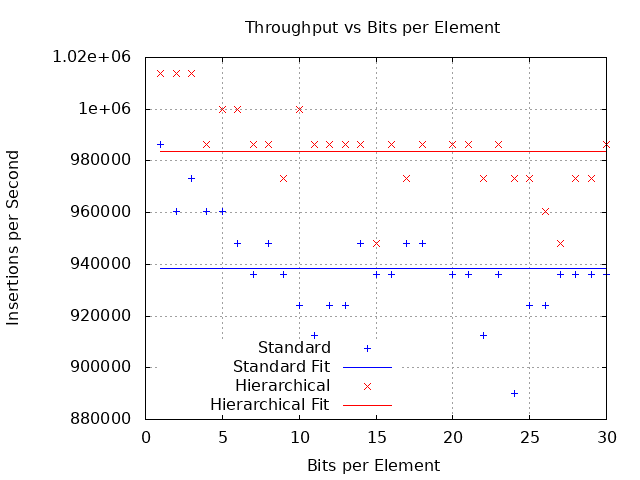
\includegraphics[width=14cm]{aol_thru.png}
\end{center}

As we can see, the hierarchical implementation does noticably better than the standard implementation. 
The lines shown on the graph represents the line of best fit for the function $f(BPE) = c$. In otherwords, it represents an ``average'' throughput for each implementation.
The average throughput for the standard implementation is $938,248$ while the averge throughput for the hierarchical implementaion is $983,627$.
Our hierarchical implementation has a higher throughput by $4\%$! This difference is not as high as it was for the random data since we have many fewer entries.
The hierarchical implementation is more beneficial the more memory is used, since higher memory usage increases the liklihood of page faulting, which is considerably more harmful in the standard implementation.
However, even for smaller uses, our implementation outpaces the standard implementation!

\begin{center}
    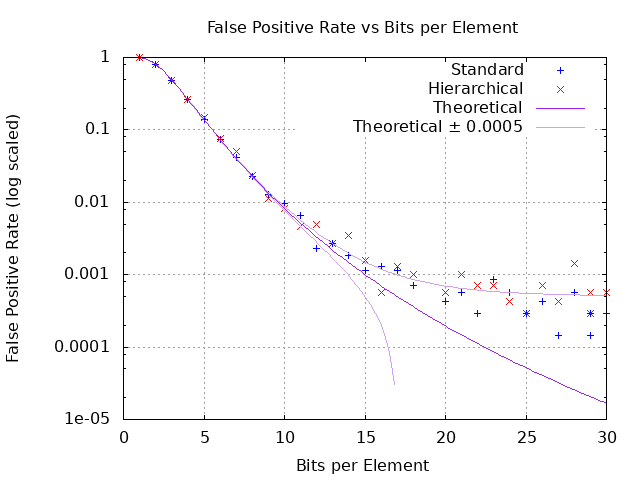
\includegraphics[width=14cm]{aol_fp.png}
\end{center}

Notice that both implementations don't perfectly match the theoretical expectation, but this can be mainly attributed to the small sample size we used to measure the false positive rate.
More importantly,the hierarchical and standard implementation have a similar false positive rate. 

\subsection{Conclusion}
Our results are positive and we hav demonstrated that our implementation is more performant without sacrificing any effectiveness.


